\documentclass[14pt,a4paper]{scrartcl}
%\usepackage[14pt]{extsizes}
\usepackage[utf8]{inputenc}
\usepackage[english,russian,ukrainian]{babel}
\usepackage{indentfirst}
\usepackage{misccorr}
\usepackage{graphicx}
\usepackage{amsmath}
\usepackage{ upgreek }
\usepackage{ verbatim }
\usepackage{amsfonts}

\graphicspath{}
\DeclareGraphicsExtensions{.jpg}

\begin{document}
	\begin{titlepage}
		\begin{center}
			\small{Міністерство освіти та науки України}\\
			\small{Київський національний університет імені Тараса Шевченка}\\
		\end{center}
			\vspace{15em}
		\begin{center}
			\large{Звіт}\\
			\large{До лабораторної роботи №3}\\
			\large{«Побудова різницевої схеми}\\
			\large{рівняння теплопровідності»}\\
		\end{center}
			
		\vspace{10em}
		

	
		\begin{flushright}
			Студента 4 курсу\\
			Факультету кібернетики\\
			Групи ОМ-4\\
			Кравця Олексія\\
			
		\end{flushright}
		
		\vspace{\fill}

		
		\begin{center}
			\small{Київ, 2019}
		\end{center}
	
	\end{titlepage}


	\newpage


\section{Постановка задачі}

Визначити час, після якого тепмература в середині мідної кулі діаметром $10 \text{см}$ дорівнюватиме $10 ^\circ C$, якщо поверхня кулі підтримується при нульовій температурі, а початкова температура кулі дорівнює $50 ^\circ C$. Фізичні характеристики мідної кулі мають $\lambda = 398 \frac{\text{Вт}}{\text{м}\cdot \text{К}}$, $c = 0.38 \frac{\text{кДж}}{\text{кг} \cdot \text{К}}$, $\rho = 8900 \frac{\text{кг}}{\text{м}^3}$.

\section{Теоретична частина}

Одновимірне рівняння теплопровідності:


\begin{gather}
		\frac{\partial u}{\partial t} = \frac{1}{x^m} \frac{\partial}{\partial x} \left( x^{m} k(x,t) \frac{du}{dx} \right) - q(x,t)u + f(x,t), x \in (a,b), t > 0 \label{eq1}\\
		u(x,0) = u_{0}(x), x\in [a,b] \label{eq2}\\
		\alpha_{1}k(a,t) \frac{du(a,t)}{dx} = \beta_{1} u(a,t) - \mu_{1}(t) \label{eq3}\\				-\alpha_{2}k(b,t) \frac{du(b,t)}{dx} = \beta_{2} u(b,t) - \mu_{2}(t) \label{eq4}
\end{gather}

Якщо рівняння розглядається у циліндричних або сферичних координатах $(m=1,2)$ , то в центрі може додатися умова симетрії

\begin{equation}\label{eq5}
	\lim_{x \to 0} x^{m}k \frac{du}{dx} = 0
\end{equation}

де $k(x,t), q(x,t), f(x,t), u_{0}(x), \mu_{1}(t), \mu_{2}(t)$ задані функції; $\alpha_{k}, \beta_{k}, (k= 1,2)$ - зажані невід'ємні сталі, причому $0 < k_{0} \leq k(x,t) \leq k_{1}$, $q(x,t) \geq 0$, $\alpha_{k}^{2} + \beta_{k}^2 \neq 0, k = 1,2$, ($k_0,k_1$ - деякі сталі)

Розв'язок на сітці $\{ x_i = a + ih, h = \frac{(b-a)}{N}, i = \overline{0,N} \} \times \{ t_j = j\tau, \tau= \frac{j}{M}, j = \overline{0,M} \}$ знаходио з різницевої схеми.

\begin{equation}\label{eq6}
	\overset{\sim}{x^{m}_i}y^{j}_{t,i} = \sigma(\overset{\sim}{p_i}y^{j+1}_{\overline{x}})_{x,i} - \sigma \overset{\sim}{x^{m}_i} \overline{q_i}y^{j+1}_{i} + (1- \sigma)(\overset{\sim}{p_i}y^{j}_{\overline{x}} )_{x,i} - (1-\sigma) \overset{\sim}{x^{m}_i}\overline{q_i}y^{j}_{i} + \overset{\sim}{x^{m}_i} \overline{f_i} 
\end{equation}

\begin{equation}\label{eq7}
	y_{i}^{0} = u_{0}(x_i), i = \overline{1,N-1}, j = \overline{1,M}
\end{equation}


\begin{multline} \label{eq8}
	\sigma \alpha_{1} \overset{\sim}{p_1} y^{j+1}_{\overline{x},1} + (1-\sigma)\alpha_{1} \overset{\sim}{p_1} y^{j}_{\overline{x},1} = x_{0}^{m} \beta_{1} \sigma y^{j+1}_{0}  + (1-\sigma) \beta_{1} x_{0}^{m} y_{0}^{j} \\- x_{0}^{m}\overline{\mu_{1}} + \frac{h}{2}\alpha_{1}\overset{\sim}{x^{m}_0} y_{t,0}^{j} - \frac{h}{2} \alpha_{1} \overset{\sim}{x^{m}_0} (\overline{f_0} -\sigma \overline{q_0}y_{0}^{j+1} + (1-\sigma)\overline{q_0} y^{j}_0 )
\end{multline}


\begin{multline} \label{eq9}
	\sigma \alpha_{2} \overset{\sim}{p_N} y^{j+1}_{\overline{x},N} + (1-\sigma)\alpha_{2} \overset{\sim}{p_N} y^{j}_{\overline{x},N} = x_{N}^{m} \beta_{2} \sigma y^{j+1}_{N}  + (1-\sigma) \beta_{2} x_{N}^{m} y_{N}^{j} \\- x_{N}^{m}\overline{\mu_{2}} + \frac{h}{2}\alpha_{2}\overset{\sim}{x^{m}_N} y_{t,N}^{j} - \frac{h}{2} \alpha_{2} \overset{\sim}{x^{m}_N} (\overline{f_N} -\sigma \overline{q_N}y_{N}^{j+1} + (1-\sigma)\overline{q_N} y^{j}_N )
\end{multline}

\begin{gather}
	\overset{\sim}{x^{m}_{0}} = h^{-1} \int_{x_0}^{x_1} x^m dx \label{eq10}\\
	\overset{\sim}{x^{m}_{N}} = h^{-1} \int_{x_{N-1}}^{x_N} x^m dx \label{eq11}\\
	\overset{\sim}{x^{m}_{i}} = (2h)^{-1} \int_{x_{i-1}}^{x_{i+1}} x^m dx \label{eq12}\\
	\overset{\sim}{p_i} = x^{m}_{i-\frac{1}{2}} \overline{k_{1-\frac{1}{2}}} \label{eq13}
\end{gather}

\newpage

\section{Практична частина}

Рівняння поставленної задачі:

\begin{gather}
	c\rho \frac{du}{dt} = \frac{\lambda}{x^2} \frac{\partial}{\partial}\left( x^2 \frac{\partial u}{\partial x}\right), x \in (0,R), t>0 \label{eq14} \\
	u(x,0) = 50, x\in [0,R] \label{eq15}\\
	\lim_{x \to 0} x^{2}\frac{\partial u}{\partial x} = 0, t>0\label{eq16} \\
	u(R, t) = 0 , t>0 \label{eq17}	
\end{gather}

де $R = 0.05 \text{м}$, $u_{kp} = 50^\circ C$. Введемо безрозмірні змінні

\begin{gather}
	\nu(x,t) = \frac{u(x,t) - u_{kp}}{u_{kp}} \label{eq18}\\
	t_1 = \frac{\lambda t}{c \rho R^2} \label{eq19}\\
	x_1 = \frac{x}{R} \label{eq20}
\end{gather}

Отримали задачу відносно $\nu(x_1, t_1)$:

\begin{gather}
	\frac{\partial \nu(x,t)}{\partial t_{1}} =  \frac{1}{x^{2}_1} \frac{\partial}{\partial x_{1}}\left( x_{1}^{2} \frac{\partial u}{\partial x_1}\right), x_1 \in (0,1), t_1 >0 \label{eq21} \\
	\nu(x_1, 0) = \frac{u(x,0) - u_{kp}}{u_{kp}} = 0 , x_{1} \in [0,1] \label{eq22} \\
	\lim_{x_1 \to 0} x_{1}^{2} \frac{\partial \nu}{\partial x_1} = 0 , t>0 \label{eq23} \\
	\nu(1,t) = \frac{u(R,t) - u_{kp}}{u_{kp}} = -1 , t>0 \label{eq24}
\end{gather}

Умовою зупинки алгоритму буде $\nu(0,t_{end}) = -\frac{4}{5}$, знайдене $t_{end}$ - це відповідь.

Застосіємо схему Кранка-Ніколсона $\sigma = 0.5$, з кроками $\tau = 0.001, h = 0.01$.

\begin{figure}[h!]
	\center{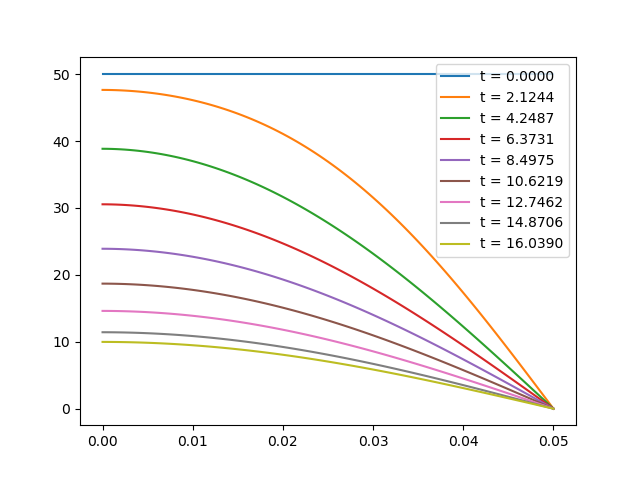
\includegraphics[scale=0.9]{Figure_1.png}}
	\caption{$ \sigma = 0.5, h = 0.01, \tau = 0.001$}
	\label{fig:image}
\end{figure}\newpage

Програма виконується за $755$ кроків, $t_{end} = 16.0390$ секунд.


\newpage
\section{Практична частина}

Будемо розглядати задачу на діаметрі кулі.
Рівняння поставленної задачі:

\begin{gather}
c\rho \frac{du}{dt} = \frac{\lambda}{x^2} \frac{\partial}{\partial}\left( x^2 \frac{\partial u}{\partial x}\right), x \in (0,R), t>0 \label{eq25} \\
u(x,0) = 50, x\in [0,R] \label{eq26}\\
u(0, t) = 0, t>0\label{eq27} \\
u(R, t) = 0 , t>0 \label{eq28}	
\end{gather}

де $R = 0.1 \text{м}$, $u_{kp} = 50^\circ C$. Введемо безрозмірні змінні

\begin{gather}
\nu(x,t) = \frac{u(x,t) - u_{kp}}{u_{kp}} \label{eq29}\\
t_1 = \frac{\lambda t}{c \rho R^2} \label{eq30}\\
x_1 = \frac{x}{R} \label{eq31}
\end{gather}

Отримали задачу відносно $\nu(x_1, t_1)$:

\begin{gather}
\frac{\partial \nu(x,t)}{\partial t_{1}} =  \frac{1}{x^{2}_1} \frac{\partial}{\partial x_{1}}\left( x_{1}^{2} \frac{\partial u}{\partial x_1}\right), x_1 \in (0,1), t_1 >0 \label{eq32} \\
\nu(x_1, 0) = \frac{u(x,0) - u_{kp}}{u_{kp}} = 0 , x_{1} \in [0,1] \label{eq33} \\
\nu(0, t) = -1 , t>0 \label{eq34} \\
\nu(1,t) = \frac{u(R,t) - u_{kp}}{u_{kp}} = -1 , t>0 \label{eq35}
\end{gather}

Умовою зупинки алгоритму буде $\nu(0.5,t_{end}) = -\frac{4}{5}$, знайдене $t_{end}$ - це відповідь.

Застосіємо схему Кранка-Ніколсона $\sigma = 0.5$, з кроками $\tau = 0.001, h = 0.01$.

\begin{figure}[h!]
	\center{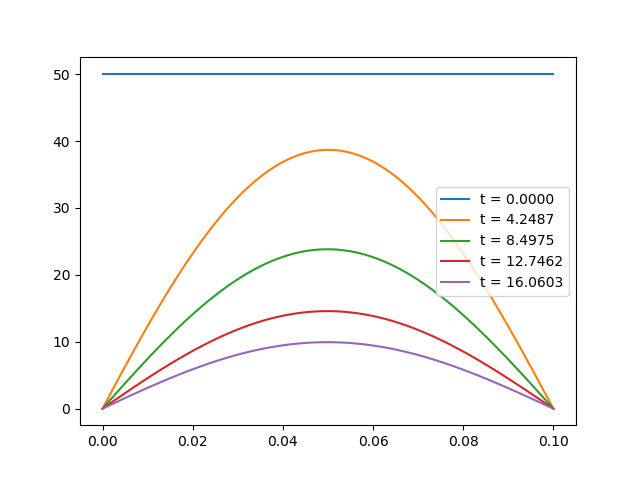
\includegraphics[scale=0.9]{Figure_2.png}}
	\caption{$ \sigma = 0.5, h = 0.01, \tau = 0.001$}
	\label{fig:image}
\end{figure}

Програма виконується за $189$ кроків, $t_{end} = 16.0603$ секунд.




\end{document}